\subsection{Análisis de desempeño}

El objetivo del análisis de desempeño es evaluar si el mismo es afectado por el paralelismo que otorga Apache Spark. El cluster de prueba consiste en un cluster local, por lo cual el paralelismo será realizado modificando la cantidad de núcleos CPU que se le provee al cluster Hadoop local. Esta configuración puede ser extrapolada fácilmente a un cluster de computadoras con más de un nodo, y con varios ejecutores por nodo.

\bigskip Las pruebas son realizadas ejecutando los experimentos de forma local y variando la configuración del contexto Spark. Ya que en este trabajo, la etapa de clustering no se realizó utilizando Apache Spark, no es detallada en esta sección. Se analizan entonces, la etapa de cálculo de similaridad, el ensamble de clustering y luego la ejecución total de los experimentos, con tamaños de muestra 100, 500 y 1000 pares de preguntas. Cada una de las ejecuciones, se realizan utilizando dos técnicas de similaridad (TF y TFIDF), para luego ensamblarlas. Además, con cada una de ellas, se realizó un algoritmo de clustering con \(k = 5\) y \(20\) ejecuciones del mismo. Las pruebas de rendimiento se realizaron con el siguiente equipo:

\begin{verbatim}
Modelo: MacBook Pro
Procesador: Intel Core i7
Velocidad del procesador: 2.6 GHz
Numero de nucleos: 6
Caché L2 (por núcleo): 256 KB
Caché L3: 12 MB
Tecnología Hyper-Threading: Habilitada
Memoria: 16 GB RAM
Almacenamiento: APPLE SSD AP0512M
\end{verbatim}

\bigskip La cantidad de núcleos de CPU asignados al contexto Spark variará de 1 a 12. La \textbf{Tabla \ref{tab:calc-matrices-sim}} 0 muestra los el tiempo total para la etapa de cálculo de matrices de similaridad, y una estimación de cálculos/segundo siendo la cantidad de cálculos total de \(2n^2-n\) por cada una de las matrices de similaridad generadas (dos en total en las pruebas de desempeño). La \textbf{Tabla \ref{tab:calc-ensamble}} muestra los tiempos para la etapa de ensamble de clustering, y una estimación de cálculos/segundo siendo la cantidad de cálculos total de \(N^2n^2\) siendo \(N\) la cantidad de ejecuciones del algoritmo de clustering en total. Para finalizar, la \textbf{Tabla \ref{tab:calc-total}}  muestra los tiempos totales de cada una de las ejecuciones. El tiempo total está compuesto un tiempo de preprocesamiento, cálculos de similaridades, algoritmos de clustering y ensamble de clustering\footnote{Detalles de los tiempos de ejecución en la tabla X.X.X.}. La cantidad estimada de calculos total, es la sumatoria de los dos explicados anteriormente más una cantidad estimada para las ejecuciones del algoritmo de clustering \(Nnki\), donde \(N=40\) ejecuciones, \(k=5\) clusters para \(i=300\) iteraciones.

\begin{table}[]
	\centering
	\begin{tabular}{|c|c|c|c|c|}
		\hline
		\multicolumn{5}{|c|}{\cellcolor[HTML]{DAE8FC}\textbf{Cálculo de matrices de similaridad}}  \\ \hline
		\cellcolor[HTML]{DAE8FC} &
		\cellcolor[HTML]{DAE8FC} &
		\cellcolor[HTML]{DAE8FC} &
		\cellcolor[HTML]{DAE8FC} &
		\cellcolor[HTML]{DAE8FC} \\
		\multirow{-2}{*}{\cellcolor[HTML]{DAE8FC}\textbf{Núcleo CPU}} &
		\multirow{-2}{*}{\cellcolor[HTML]{DAE8FC}\textbf{Tamaño de muestra}} &
		\multirow{-2}{*}{\cellcolor[HTML]{DAE8FC}\textbf{Cálculos}} &
		\multirow{-2}{*}{\cellcolor[HTML]{DAE8FC}\textbf{Tiempo}} &
		\multirow{-2}{*}{\cellcolor[HTML]{DAE8FC}\textbf{Calc/seg}} \\ \hline
		1  & 100   & 39996   & 62.990                           & 634.957                          \\ \hline
		2  & 100   & 39996   & 46.081                           & 867.955                          \\ \hline
		4  & 100   & 39996   & 33.074                           & 1209.303                         \\ \hline
		8  & 100   & 39996   & 31.276                           & 1278.827                         \\ \hline
		12 & 100   & 39996   & 32.336                           & 1236.882                         \\ \hline
		1  & 500   & 999996  & 763.889                          & 1309.086                         \\ \hline
		2  & 500   & 999996  & 576.669                          & 1734.091                         \\ \hline
		4  & 500   & 999996  & 402.376                          & 2485.226                         \\ \hline
		8  & 500   & 999996  & 324.826                          & 3078.561                         \\ \hline
		12 & 500   & 999996  & 328.300                          & 3045.980                         \\ \hline
		1  & 1,000 & 3999996 & 2950.810                         & 1355.559                         \\ \hline
		2  & 1,000 & 3999996 & 2073.179                         & 1929.402                         \\ \hline
		4  & 1,000 & 3999996 & \multicolumn{1}{r|}{1423.895968} & \multicolumn{1}{r|}{2809.191184} \\ \hline
		8  & 1,000 & 3999996 & \multicolumn{1}{r|}{1176.5926}   & \multicolumn{1}{r|}{3399.644023} \\ \hline
		12 & 1,000 & 3999996 & \multicolumn{1}{r|}{1253.433926} & \multicolumn{1}{r|}{3191.230042} \\ \hline
	\end{tabular}
	\caption{Cálculos aproximados y tiempo para la etapa de cálculo de matrices de similaridad para los distintos tamaños de muestra.}
	\label{tab:calc-matrices-sim}
\end{table}

\begin{table}[]
	\centering
	\begin{tabular}{|c|c|c|c|c|}
		\hline
		\multicolumn{5}{|c|}{\cellcolor[HTML]{DAE8FC}\textbf{Ensamble de Clustering}} \\ \hline
		\cellcolor[HTML]{DAE8FC} &
		\cellcolor[HTML]{DAE8FC} &
		\cellcolor[HTML]{DAE8FC} &
		\cellcolor[HTML]{DAE8FC} &
		\cellcolor[HTML]{DAE8FC} \\
		\multirow{-2}{*}{\cellcolor[HTML]{DAE8FC}\textbf{Núcleo CPU}} &
		\multirow{-2}{*}{\cellcolor[HTML]{DAE8FC}\textbf{Tamaño de muestra}} &
		\multirow{-2}{*}{\cellcolor[HTML]{DAE8FC}\textbf{Cálculos}} &
		\multirow{-2}{*}{\cellcolor[HTML]{DAE8FC}\textbf{Tiempo}} &
		\multirow{-2}{*}{\cellcolor[HTML]{DAE8FC}\textbf{Calc/seg}} \\ \hline
		1        & 100         & 16000000        & 15.978         & 1001359.283       \\ \hline
		2        & 100         & 16000000        & 10.388         & 1540193.812       \\ \hline
		4        & 100         & 16000000        & 6.872          & 2328158.952       \\ \hline
		8        & 100         & 16000000        & 6.309          & 2536184.216       \\ \hline
		12       & 100         & 16000000        & 5.698          & 2808037.305       \\ \hline
		1        & 500         & 400000000       & 40.430         & 9893694.968       \\ \hline
		2        & 500         & 400000000       & 25.684         & 15573735.642      \\ \hline
		4        & 500         & 400000000       & 21.511         & 18594808.023      \\ \hline
		8        & 500         & 400000000       & 18.017         & 22201723.864      \\ \hline
		12       & 500         & 400000000       & 15.737         & 25417188.196      \\ \hline
		1        & 1,000       & 1600000000      & 95.886         & 16686498.744      \\ \hline
		2        & 1,000       & 1600000000      & 58.053         & 27560883.672      \\ \hline
		4        & 1,000       & 1600000000      & 47.732525      & 33520120.71       \\ \hline
		8        & 1,000       & 1600000000      & 43.265526      & 36980944.14       \\ \hline
		12       & 1,000       & 1600000000      & 43.699182      & 36613957.67       \\ \hline
	\end{tabular}
	\caption{Cálculos aproximados y tiempo para la etapa de ensamble de clustering para los distintos tamaños de muestra.}
	\label{tab:calc-ensamble}
\end{table}

\begin{table}[]
	\centering
	\begin{tabular}{|c|c|c|c|c|}
		\hline
		\multicolumn{5}{|c|}{\cellcolor[HTML]{DAE8FC}\textbf{Total}} \\ \hline
		\cellcolor[HTML]{DAE8FC} &
		\cellcolor[HTML]{DAE8FC} &
		\cellcolor[HTML]{DAE8FC} &
		\cellcolor[HTML]{DAE8FC} &
		\cellcolor[HTML]{DAE8FC} \\
		\multirow{-2}{*}{\cellcolor[HTML]{DAE8FC}\textbf{Núcleo CPU}} &
		\multirow{-2}{*}{\cellcolor[HTML]{DAE8FC}\textbf{Tamaño de muestra}} &
		\multirow{-2}{*}{\cellcolor[HTML]{DAE8FC}\textbf{Cálculos}} &
		\multirow{-2}{*}{\cellcolor[HTML]{DAE8FC}\textbf{Tiempo}} &
		\multirow{-2}{*}{\cellcolor[HTML]{DAE8FC}\textbf{Calc/seg}} \\ \hline
		1    & 100     & 40039996     & 88.554        & 452154.152   \\ \hline
		2    & 100     & 40039996     & 64.830        & 617610.886   \\ \hline
		4    & 100     & 40039996     & 47.607        & 841058.532   \\ \hline
		8    & 100     & 40039996     & 45.024        & 889313.092   \\ \hline
		12   & 100     & 40039996     & 44.428        & 901233.021   \\ \hline
		1    & 500     & 520999996    & 828.022       & 629210.531   \\ \hline
		2    & 500     & 520999996    & 624.102       & 834799.734   \\ \hline
		4    & 500     & 520999996    & 446.984       & 1165589.860  \\ \hline
		8    & 500     & 520999996    & 363.617       & 1432826.642  \\ \hline
		12   & 500     & 520999996    & 362.982       & 1435333.416  \\ \hline
		1    & 1,000   & 1843999996   & 3106.846      & 593527.943   \\ \hline
		2    & 1,000   & 1843999996   & 2199.752      & 838276.366   \\ \hline
		4    & 1,000   & 1843999996   & 1530.309932   & 1204984.662  \\ \hline
		8    & 1,000   & 1843999996   & 1282.804328   & 1437475.658  \\ \hline
		12   & 1,000   & 1843999996   & 1370.473092   & 1345520.76   \\ \hline
	\end{tabular}
	\caption{Cálculos aproximados y tiempos totales para los distintos tamaños de muestra.}
	\label{tab:calc-total}
\end{table}

Graficando las tablas \ref{tab:calc-matrices-sim} y \ref{tab:calc-ensamble} para cada uno de los tamaños de muestra de forma sumarizada, se puede ver claramente como el desempeño aumenta hasta cierto nivel de paralelismo. En un cluster Spark, existe una cota superior al número de nodos/ejecutores/CPU en el cual más allá del mismo, el aumento del desempeño es marginal. Este límite depende de la naturaleza de la aplicación y difiere notablemente si la misma hace uso intensivo de CPU o uso intensivo de operaciones de entrada-salida.

\begin{figure}
	\centering
	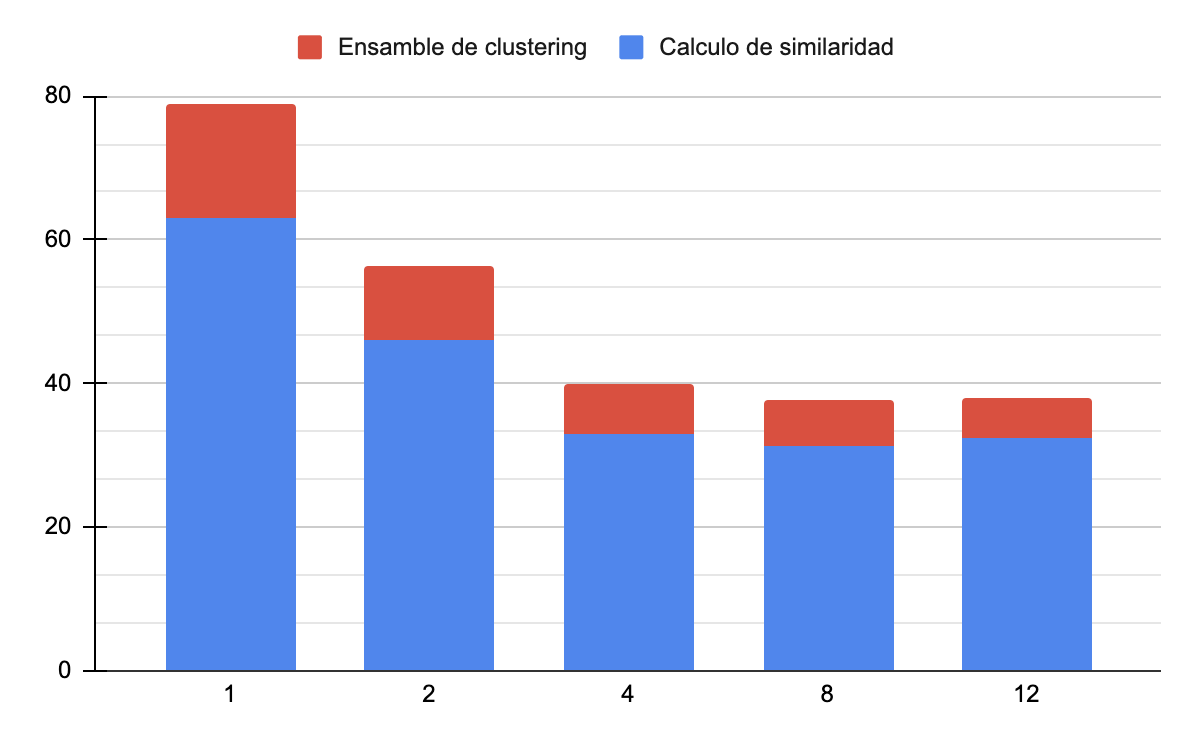
\includegraphics[width=0.7\linewidth]{10_resultados/imagenes/performance_100}
	\caption{Tiempos en segundos para ejecuciones de tamaño de muestra de 100 pares de preguntas y distintos núcleos de CPU.}
	\label{fig:performance100}
\end{figure}

\begin{figure}
	\centering
	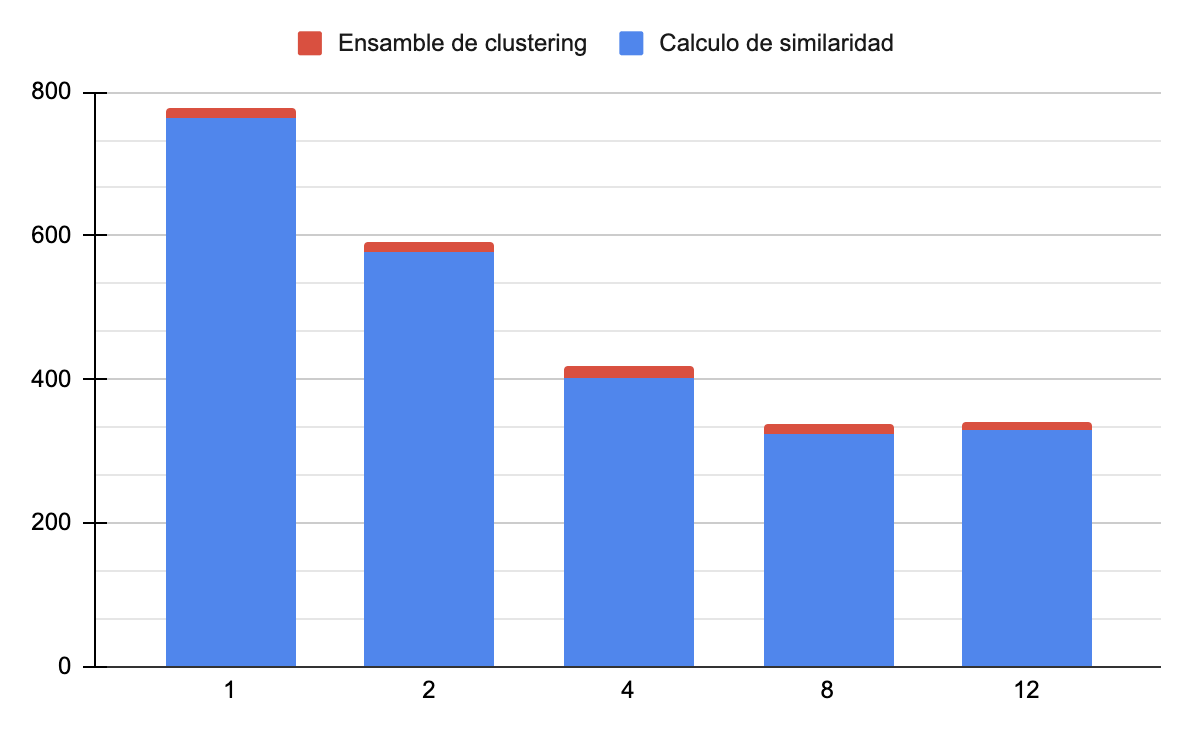
\includegraphics[width=0.7\linewidth]{10_resultados/imagenes/performance_500}
	\caption{Tiempos en segundos para ejecuciones de tamaño de muestra de 500 pares de preguntas y distintos núcleos de CPU.}
	\label{fig:performance500}
\end{figure}

\begin{figure}
	\centering
	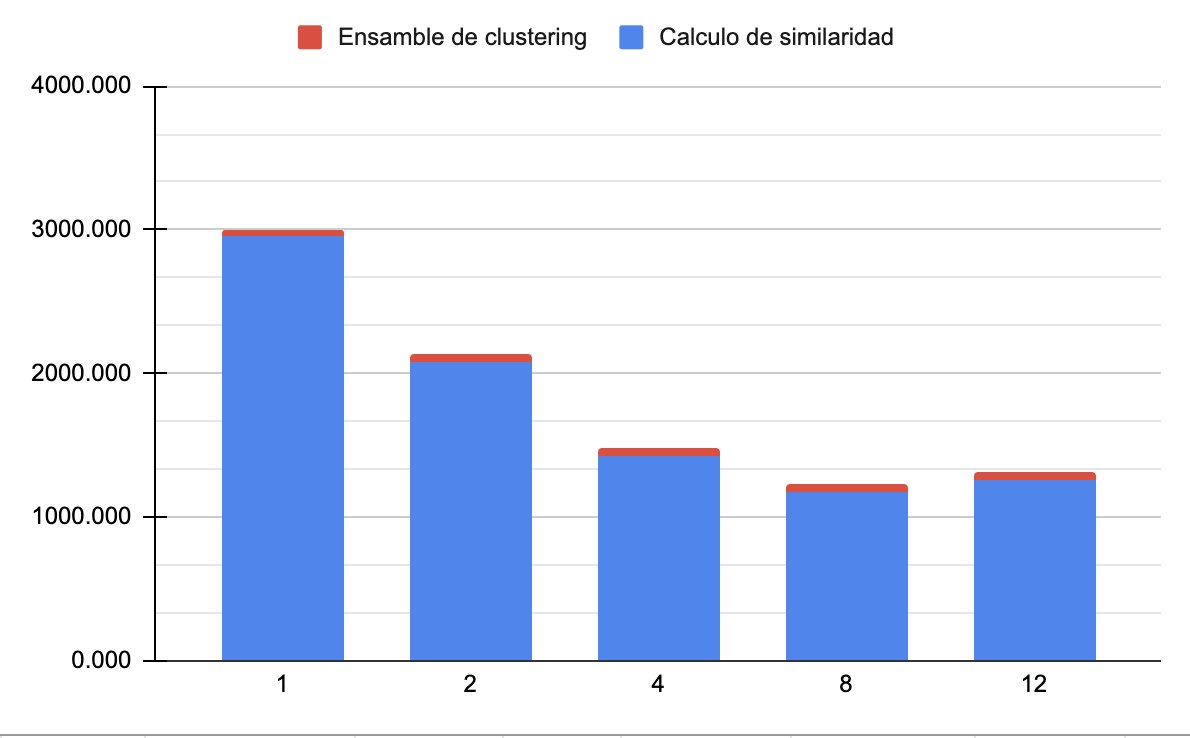
\includegraphics[width=0.7\linewidth]{10_resultados/imagenes/performance_1000}
	\caption{Tiempos en segundos para ejecuciones de tamaño de muestra de 1000 pares de preguntas y distintos núcleos de CPU.}
	\label{fig:performance1000}
\end{figure}

\bigskip El tiempo total de ejecución del método EQuAL decrece exponencialmente configurando un correcto nivel de paralelismo. Por lo cual, la arquitectura propuesta provee un método sencillo para escalar horizontalmente y poder procesar grandes cantidades de datos de forma eficiente. La configuración óptima del cluster de computadoras que soportará la arquitectura depende del tamaño del conjunto de datos de entrada.
